\newcommand{\ClassPath}{../../yukibook.cls}
\documentclass{\ClassPath/yukibook}


\begin{document}

    \yukibook{Sistemas en nube pública: AWS} % Title
    {Rubén Gómez Olivencia}  % Author
    {2023-2024}    % Year
    {} % Name of degree
    {} % catch phrase
    {} % the phrase's author
    {img/aws.png} %cover
    {252f3e}
    {aws} %mini-title

    \coverpage
    \graphicspath{{../../yukibook.cls/}}
    \licensepage

    \tableofcontents

    %--------------------------------------------------------------------------
    % Start your parts, chapters and sections here
    %--------------------------------------------------------------------------
    \graphicspath{{img/}}

    \part{Cloud Computing}
    \chapter{Introducción}

Los servicios que utilizamos al navegar por internet, al consultar páginas web o al utilizar \textit{apps} en el móvil, realmente están alojados en un conjunto de ordenadores (denominados \textbf{servidores}) que están almacenados en un \textbf{CPD} (centro de procesamiento de datos).

Hace unos años había empresas pequeñas que contaban con sus propios servidores en sus oficinas, abaratando parte del coste del mantenimiento de los servidores, ya que no tenían que alquilar el espacio o el propio servidor. Si se quedaba pequeño, compraban uno nuevo, o reajustaban los recursos.

Con el avance de internet, han ido surgiendo distintos proveedores que ofrecen servicios para que las empresas puedan contratarlos en condiciones más favorables y en CPDs profesionales. Veremos diferentes tipos de computación y diferenciaremos distintos tipos de “computación en la nube”.



\chapter{Sistemas de computación propios}
Dado que tener el servidor en una oficina puede suponer distintos riesgos (pérdida de electricidad, robo de datos, acceso al servidor por parte de personas no autorizadas, tener la necesidad de tener IP estática en la oficina,...), muchas empresas deciden delegar la parte pública de sus servicios en empresas que cumplen con estándares de seguridad para tener servidores de manera segura.

\infobox{Se siguen teniendo servidores en las oficinas, pero son para tareas internas, de desarrollo o para el control de dominios. \textbf{No es habitual tener servicios externos}.}

Para los servicios externos, dependiendo del tamaño de la empresa, hoy en día lo habitual es delegar parte del mantenimiento o de los servicios en un proveedor externo.

Algunos ejemplos de sistemas de computación propios (cuando nos referimos a \textit{hardware} propio) puede ser:

\begin{itemize}
    \item \textbf{CPD propio}: Esto sólo está al alcance de empresas muy grandes, que necesitan de muchos servidores y que tienen la necesidad de montar su propio CPD parar sus propios servicios.

    \item \textbf{Alquiler de un \textit{rack} en un CPD profesional}: Existen empresas que se encargan de crear CPDs donde alquilan armarios donde poder colocar nuestros servidores físicos. La empresa nos proporcionará el espacio, el ancho de banda que contratemos, y puede que otros servicios extra de red (\textit{firewall} perimetral, sistemas para apaciguar ataques de denegación de servicios...). Por otro lado, el \textit{hardware} del servidor lo proporcionaremos nosotros, y cualquier posible rotura del mismo será cosa nuestra.

    En este tipo de sitios se necesita pedir cita previa para acceder a los servidores, y sólo ciertas personas pre-autorizadas previamente podrán entrar. 

    \item \textbf{Alquiler de máquinas virtuales}: Con el \textbf{\textit{boom}} de la virtualización, surgieron compañías que ofrecen la posibilidad de contratar unos recursos (con computación, RAM y almacenamiento limitados) que están virtualizados dentro de la infraestructura del proveedor. Esto hace que sea barato de contratar, pero toda la gestión del sistema operativo y del software sea por nuestra cuenta.
\end{itemize}


Dependiendo de las necesidades de la empresa, se hará uso de un sistema u otro. El problema en estos casos, es que normalmente es necesario un equipo de informáticos que tengan los conocimientos adecuados dependiendo del tipo de infraestructura que tengamos.

Aunque hoy en día este tipo de computación sigue siendo barato y funcional, el término “computación en la nube” ha hecho que este tipo de contrataciones hayan quedado en parte relegadas.



\chapter{Computación en la nube}

La computación en la nube se puede resumir como el uso de una red de servidores al que de manera remota se puede solicitar una serie de recursos que nos proporcionará de manera casi instantánea, y sin la gestión activa por nuestra parte. Normalmente \textbf{la gestión de todo se puede realizar a través de un panel web de configuración}.

En lugar de solicitar un recurso físico como tal, “la nube”, que está compuesta por un conjunto de servidores que ha sido configurada como “un todo”, es capaz de proporcionarnos distintos tipos de recursos dependiendo de las necesidades que tengamos en ese momento.

Por poner sólo unos ejemplos:

\begin{itemize}
    \item \textbf{Software as a Service} (SaaS): En este caso se contrata lo necesario para poder hacer uso de un software y todo los datos que se vayan a almacenar con él. El proveedor nos da acceso a una instancia del software que está configurada y que permitirá el uso con unos recursos limitados. 
    
    De esta manera, no nos tendremos que preocupar del \textit{hardware} en el que está instalado, o la propia instalación del software. \textbf{Ejemplos}: servicio blog; sistema ERP para una empresa; sistema de base de datos con alta disponibilidad y \textit{backups} incluidos... 

    \item \textbf{Platform as a service} (PaaS): Se nos proporcionará una plataforma donde podremos desplegar o correr el servicio que configuremos por nuestra cuenta. El ejemplo más habitual es el de obtener una máquina virtual donde podremos desplegar el servicio que nos interese instalar.
    
    La ventaja del PaaS es que no nos tenemos que preocupar en qué \textit{hardware} está corriendo, y que en caso de necesidad, podríamos ampliar los recursos de manera sencilla. Como desventaja, es que el coste puede volverse muy elevado y en algunos casos complejo de calcular.
    
    \item \textbf{Infraestructure as a Service} (IaaS): Cuando nos referimos a “Infraestructura” hace referencia a un conjunto de servicios como son la red, el almacenamiento, servidores, virtualización, servicios... El proveedor nos proporcionará un conjunto de servicios que es equiparable a tener una red propia con nuestros propios servidores y servicios.
    
    A la hora de mantener y desplegar este tipo de arquitectura, debemos tener los conocimientos adecuados para saber qué se está realizando. Los proveedores facilitan la labor de realizar los despliegues, pero es tarea de quien realiza la acción de conocer exactamente qué se está haciendo y el coste que tendrá.
\end{itemize}


\chapter{Tipos de computación en la nube}

A la hora de hablar de computación en la nube debemos de distinguir principalmente entre dos tipos. Dependiendo del tamaño de nuestra empresa, del departamento de informática que tengamos, de los conocimientos que tengamos y/o del tiempo que tengamos para aprender, deberemos optar por una o por otra.

\section{Nube privada}

La gestión de una nube privada es aquella que está diseñada para una sola organización, y que será administrada por la propia empresa o con ayuda de terceros. Crear una infraestructura propia para la gestión de una nube privada no es una tarea sencilla, ya que va a requerir de una inversión inicial de dinero para la compra de bastante \textit{hardware}, conocimiento para administrarlo, mantenimiento, posibles cambios a futuro...

\errorbox{\textbf{Crear y mantener una nube privada no es una tarea al alcance de cualquier empresa. Es una labor compleja y cara.}}

Para poder crear una nube privada existe distinta tecnología de orquestación de servicios que se puede utilizar:

\begin{itemize}
	\item \href{https://www.openstack.org/}{Openstack}: Nos permite realizar una infraestructura de nube completa, diferenciando entre nodos de computación, de almacenamiento, ...
	
	\item \href{https://cloudstack.apache.org/}{Apache CloudStack}: permite la gestión de grandes redes de máquinas virtuales para la gestión en alta disponibilidad y alta escabilidad.
	
	\item \href{https://www.proxmox.com/en/proxmox-virtual-environment/overview}{Proxmox}: Proxmox no es un sistema de nube privada como tal, ya que es un sistema de virtualización. Por otro lado, es un sistema que permite crear clústers de nodos de virtualización de manera sencilla, por lo que puede ser utilizado como un primer punto de partida para el inicio de una nube privada.
\end{itemize}


\section{Nube pública}

Un proveedor de nube pública es aquel que ofrece los servicios de su propia infraestructura para la gestión y creación de una infraestructura propia a un cliente a través de una suscripción de pago o a través de un sistema de “pago por servicio”.

Hoy en día los proveedores de nube pública son grandes compañías que ofrecen decenas de servicios que son fácilmente contratables a través de un interfaz de administración web, o también a través de sistemas API para poder automatizar tareas.

\begin{center}
	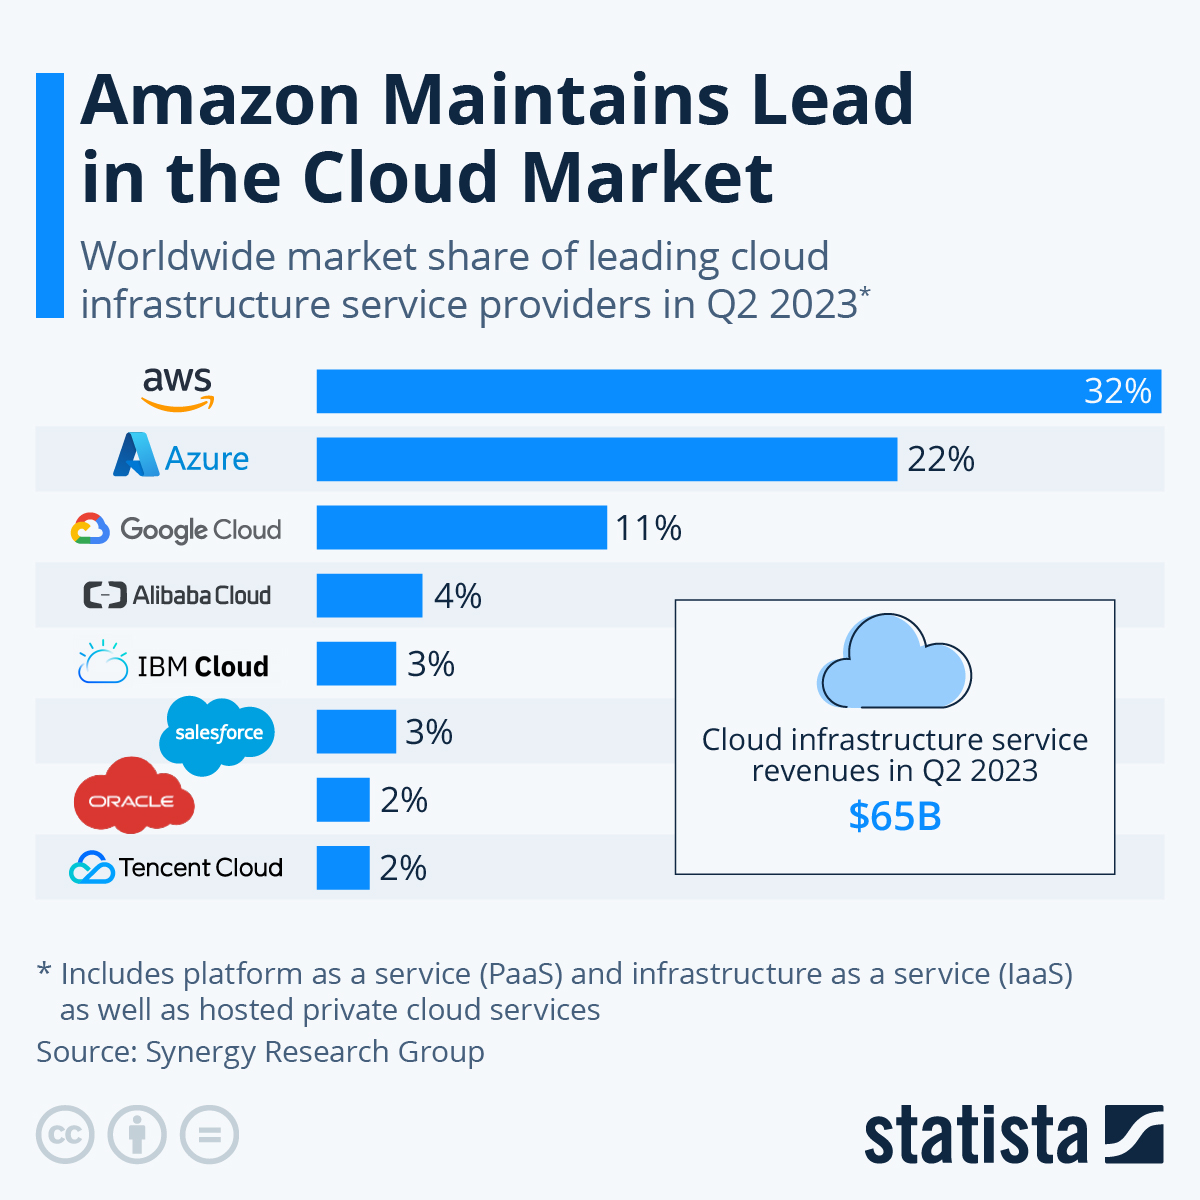
\includegraphics[frame,width=0.7\linewidth]{stats.jpeg}
	\captionof{figure}{Fuente: \href{https://www.statista.com/chart/18819/worldwide-market-share-of-leading-cloud-infrastructure-service-providers/}{Statista}}
\end{center}


Entre los proveedores más conocidos de nube pública están:

\begin{itemize}
	\item \textbf{\href{https://aws.amazon.com/es/}{Amazon Web Services}} (AWS): Aunque el negocio inicial de Amazon era el de la venta de libros \textit{online}, durante la creación de un negocio para la creación de tiendas online a terceros se dieron cuenta que sus sistemas internos no tenían la velocidad adecuada.
	
	Decidieron reimplementar toda la infraestructura utilizando estándares abiertos y el sistema \href{https://en.wikipedia.org/wiki/REST}{REST} para la comunicación. En el 2002 lanzó los primeros servicios pero el auge fue en el 2006 cuando lanzó \textbf{EC2} para la generación de máquinas virtuales.
	
	\item \textbf{\href{https://azure.microsoft.com/es-es/}{Microsoft Azure}}: Es la segunda empresa de nube pública. Aunque es la plataforma de Microsoft, Linux es el sistema más utilizado dentro de la virtualización de servicios.
	
	\item \textbf{\href{https://cloud.google.com/}{Google Cloud Platform}}: Google no se podía quedar atrás y también ofrece su sistema de nube pública. Ofrece muchos servicios y zonas de computación, y con la creación del sistema de orquestación de contenedores Kubernetes en 2015, consiguió buena cuota de mercado.
	
	\item \textbf{\href{https://www.ibm.com/cloud}{IBM / Softlayer}}: El sistema de nube público actual de IBM fue inicialmente conocido como SoftLayer, ya que posteriormente lo compró IBM. Aunque se inició en 2005, hoy en día su cuota de mercado no es muy alta.
	
	\item \textbf{\href{https://www.alibabacloud.com/}{Alibaba Cloud}}: Aunque en occidente es posible que no lo conozcamos, Alibaba es un gigante tecnológico en Asia que está detrás de AliExpress, entre otros servicios.  Su cuota de mercado es baja a nivel global, pero muy alta en Asia.
	
\end{itemize}
    
    \part{Introducción a AWS}
    \chapter{Antes de empezar}

Hay que tener en cuenta que lo que se va a explicar en este documento es el acceso a AWS Academy, por lo que existe una pequeña diferencia con una cuenta de AWS estándar, como la que se obtendría al crear una cuenta real y al introducir los datos de la tarjeta de crédito.

\href{https://aws.amazon.com/es/training/awsacademy/}{AWS Academy} ofrece a las instituciones de educación superior un plan de estudios de computación en la nube gratuito y la posibilidad de crear laboratorios personalizados, o libres, para poder realizar despliegues en un sistema de nube pública.

La ventaja de AWS Academy es que va a permitir a los alumnos a hacer uso del interfaz y de la infraestructura de AWS sin tener que hacer uso de una tarjeta de crédito. Ahora bien, \textbf{existen ciertas limitaciones} que no nos encontraríamos en una cuenta de AWS real.

Como vamos a hacer uso de la infraestructura real de AWS, para que no se abuse de ello, los laboratorios estarán limitados a una cantidad de 100\$ y de 4 horas de uso límite. A medida que vamos realizando despliegues o vamos utilizando servicios, la cantidad de dinero irá disminuyendo.

Por otro lado, para evitar que los servicios se queden corriendo (y por tanto, gasten dinero), los laboratorios tendrán un contador que al llegar a 4 horas se apagarán. \textbf{No existe problema en volver a iniciar el laboratorio, o resetear el contador}.


\chapter{Acceder a los cursos}

Para acceder a los cursos en los que el profesor nos ha matriculado, nos habrá llegado un mail que nos mandará a una página donde tendremos que indicar si tenemos ya una cuenta o tenemos que crearla:

\begin{center}
	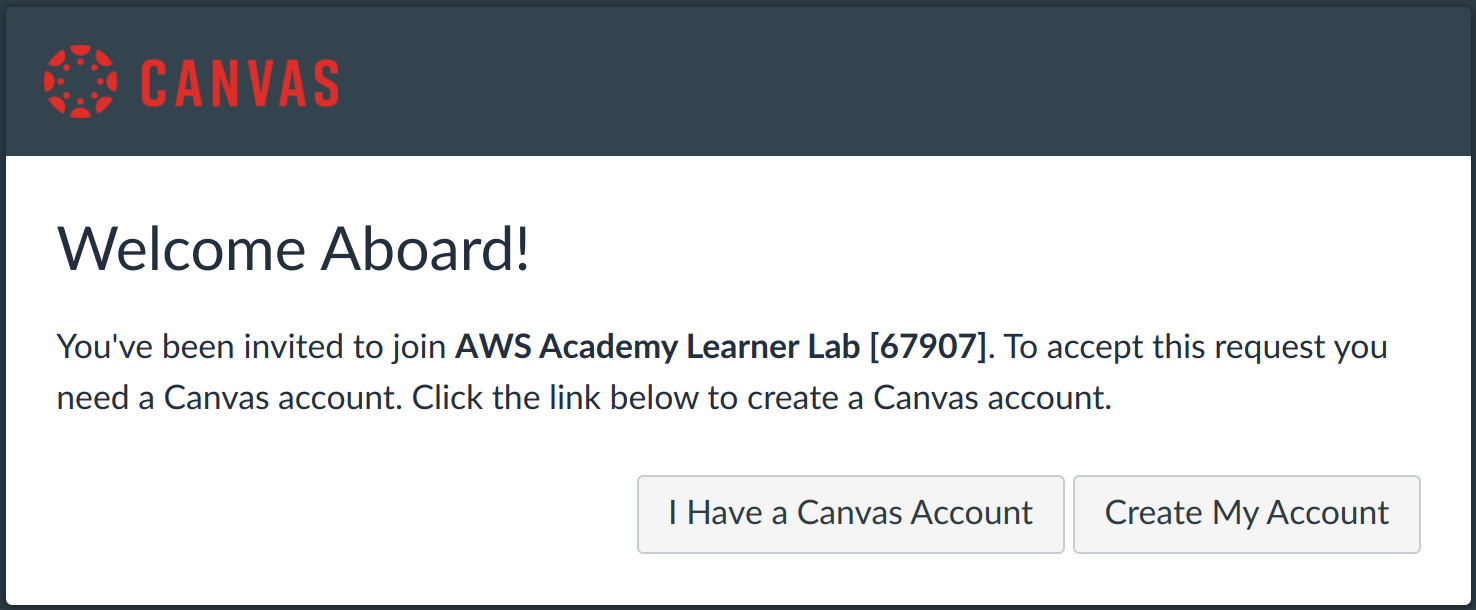
\includegraphics[width=0.7\linewidth]{create_account.png}
\end{center}

Debemos introducir una contraseña y aceptar los terminos para poder crear la cuenta. Una vez creada, nos mandará directamente al curso al que nos han matriculado.

Si ya tenemos una cuenta creada previamente, podemos ir al \href{https://www.awsacademy.com/vforcesite/LMS_Login}{panel de acceso} y elegir la opción \textbf{Student Login}. En ese punto nos aparecerá el formulario en el que debemos introducir el nombre de usuario y la contraseña.

\begin{center}
	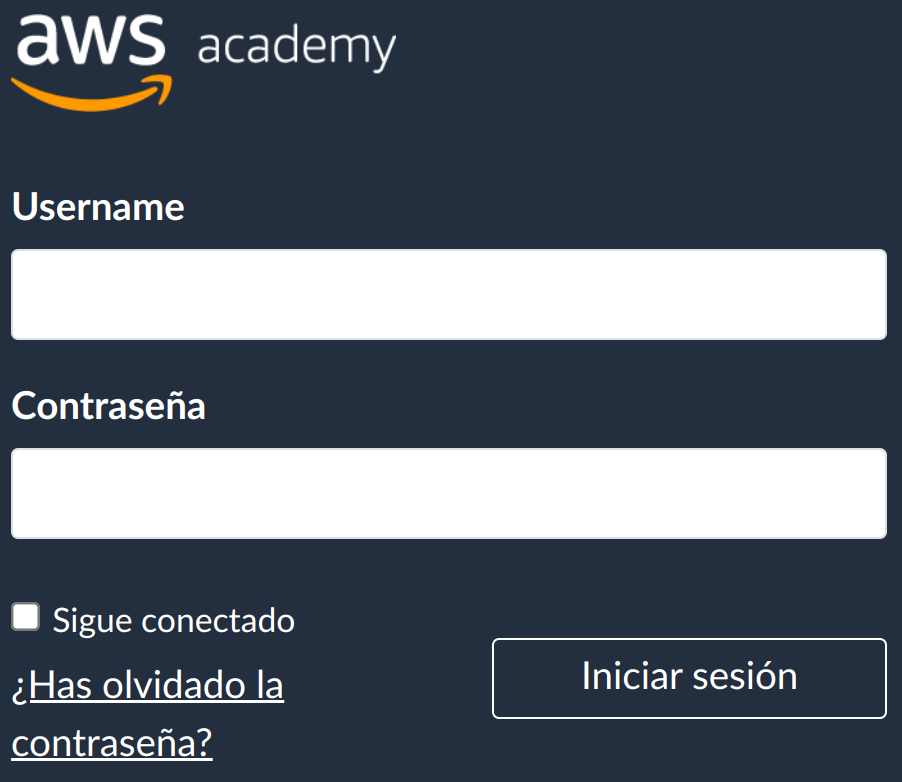
\includegraphics[width=0.5\linewidth]{login.png}
\end{center}

\chapter{Acceder al laboratorio}

Una vez logueado veremos los posibles cursos en los que estamos matriculados, y debemos ir al curso correspondiente. Una vez en el curso, luego hay que ir a “Módulos → Iniciar el Laboratorio de aprendizaje de AWS Academy”, y aparecerá una página en el que abajo del todo tendréis un botón para aceptar las condiciones de uso, y luego veremos algo similar a la siguiente pantalla:

\begin{center}
	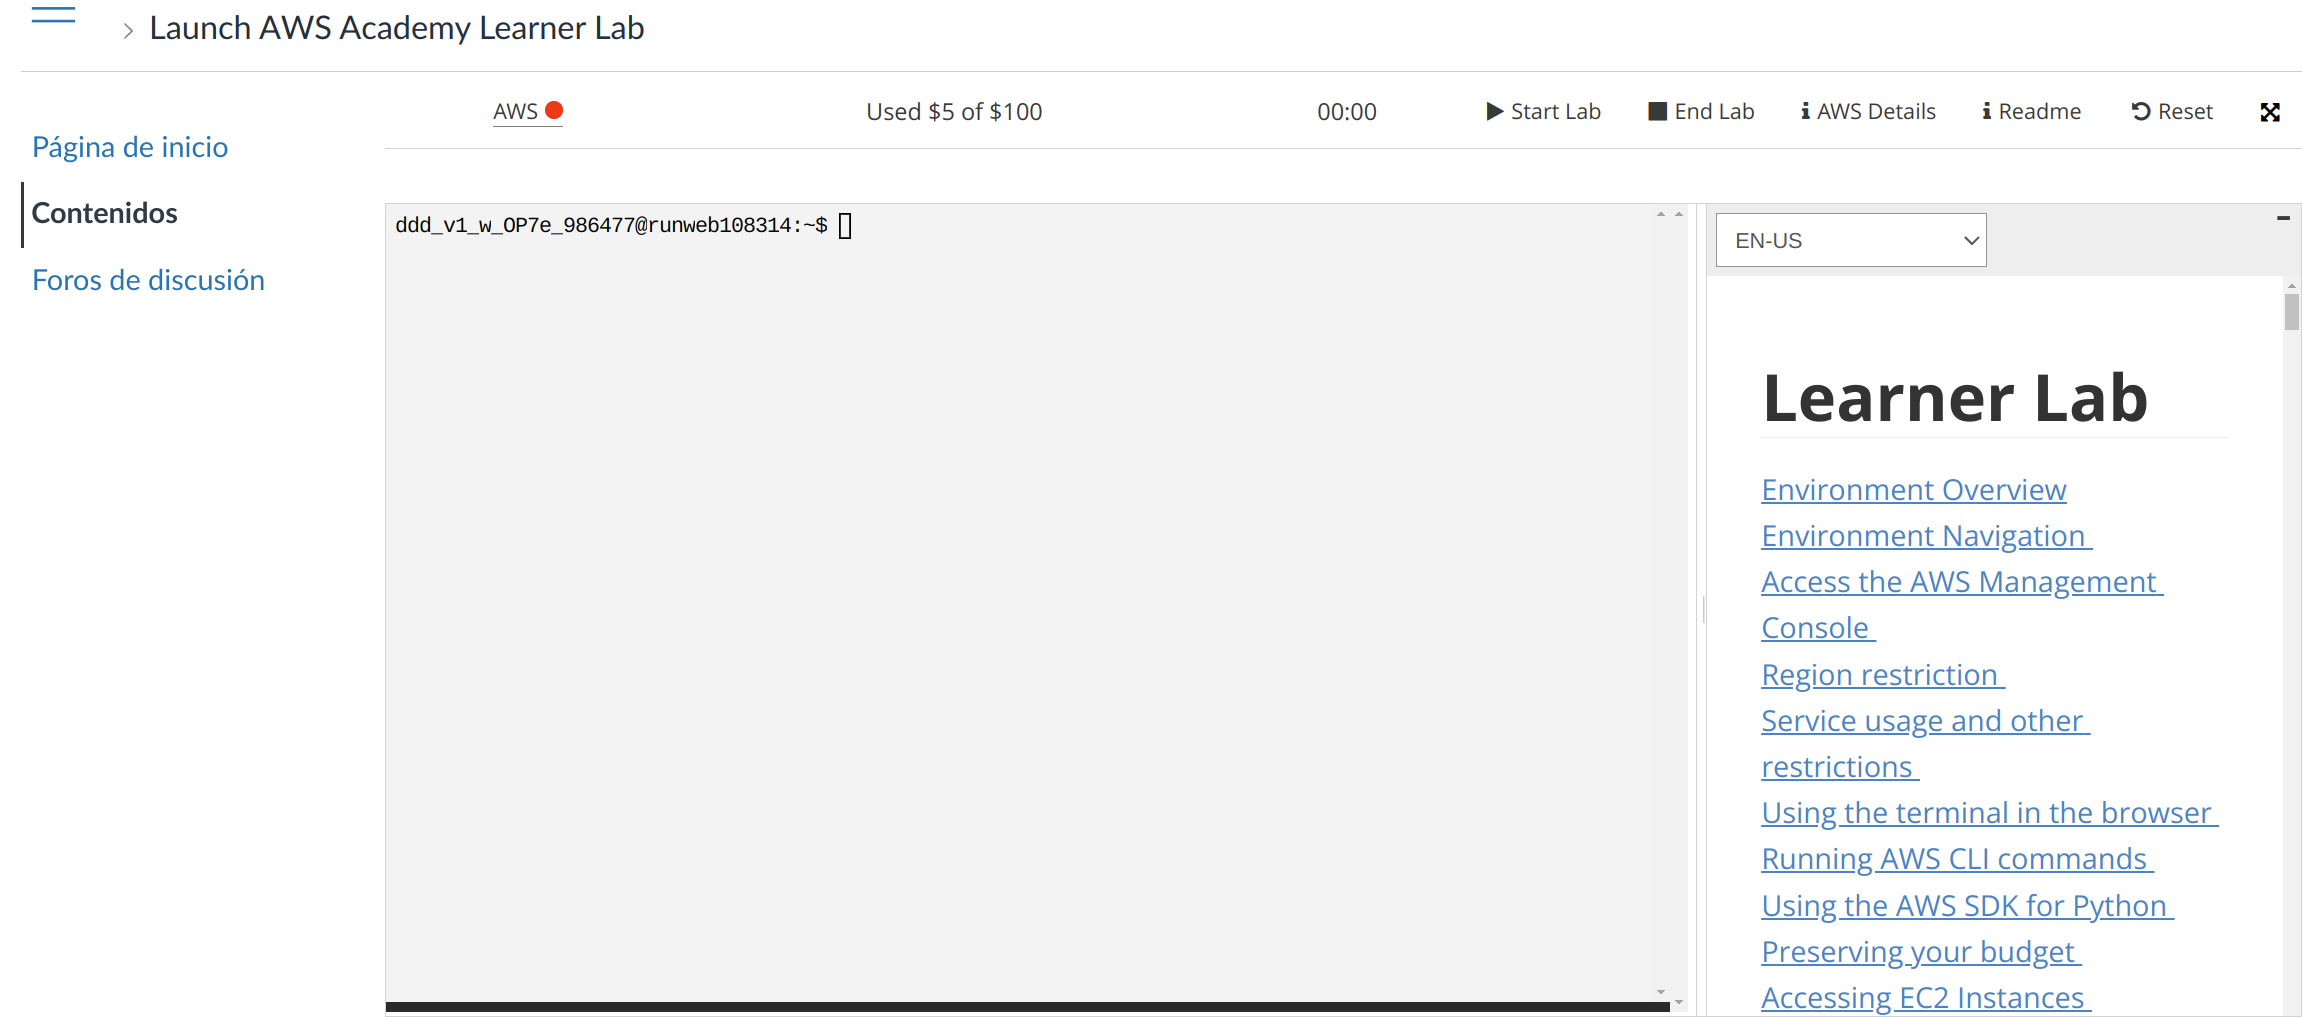
\includegraphics[frame, width=0.9\linewidth]{launcher.png}
\end{center}

En esta pantalla podemos ver distinta información del propio laboratorio y su estado:

\begin{itemize}
	\item \textbf{AWS \color{red}●}: Estado visual del laboratorio. En este caso, el círculo aparece en rojo porque el laboratorio está apagado. Al darle a iniciar, se pondrá en color amarillo ({\color{yellow}●}) mientras el laboratorio se está preparando. Cuando esté listo para ser utilizado se pondrá en verde ({\color{green}●}).
	
	\item \textbf{Used \$5 of \$100}: Cuánto dinero nos hemos gastado en el laboratorio de los 100 dólares que tenemos. Este gasto no se actualiza en tiempo real, y pueden pasar algunas horas hasta que se refleje el gasto real.
	
	\item \textbf{00:00}: El tiempo que le queda al laboratorio encendido. Es una cuenta atrás de 4 horas. 
	
	\item \faPlay  \textbf{ Start Lab}: Iniciar el laboratorio.
	
	\item \faStop  \textbf{ End Lab}: Parar el laboratorio. Todo lo realizado se para, pero hay ciertos servicios que se siguen cobrando (almacenamiento de ciertos espacios).
	
	\item \faInfo  \textbf{ AWS Details}: Detalles del laboratorio. \textbf{Más adelante hablaremos de este apartado}.
	
	\item \faInfo  \textbf{ Readme}: Tutoriales y manuales sobre el laboratorio.
	
	\item \faUndo \textbf{ Reset}: Resetea el laboratorio y borrará todo el contenido realizado. Lo deja como si estuviese recién inicializado.
\end{itemize}

El terminal que aparece es un interfaz de administración para el laboratorio, y desde el que podríamos realizar administración del laboratorio, o incluso levantar nuevos servicios a través del CLI \textbf{aws}. Por otro lado, no lo vamos a utilizar.

\warnbox{\textbf{La primera vez que encendamos el laboratorio puede tardar entre 2 y 5 minutos.}}

Cuando tenemos el laboratorio encendido la imagen será la siguiente

\begin{center}
	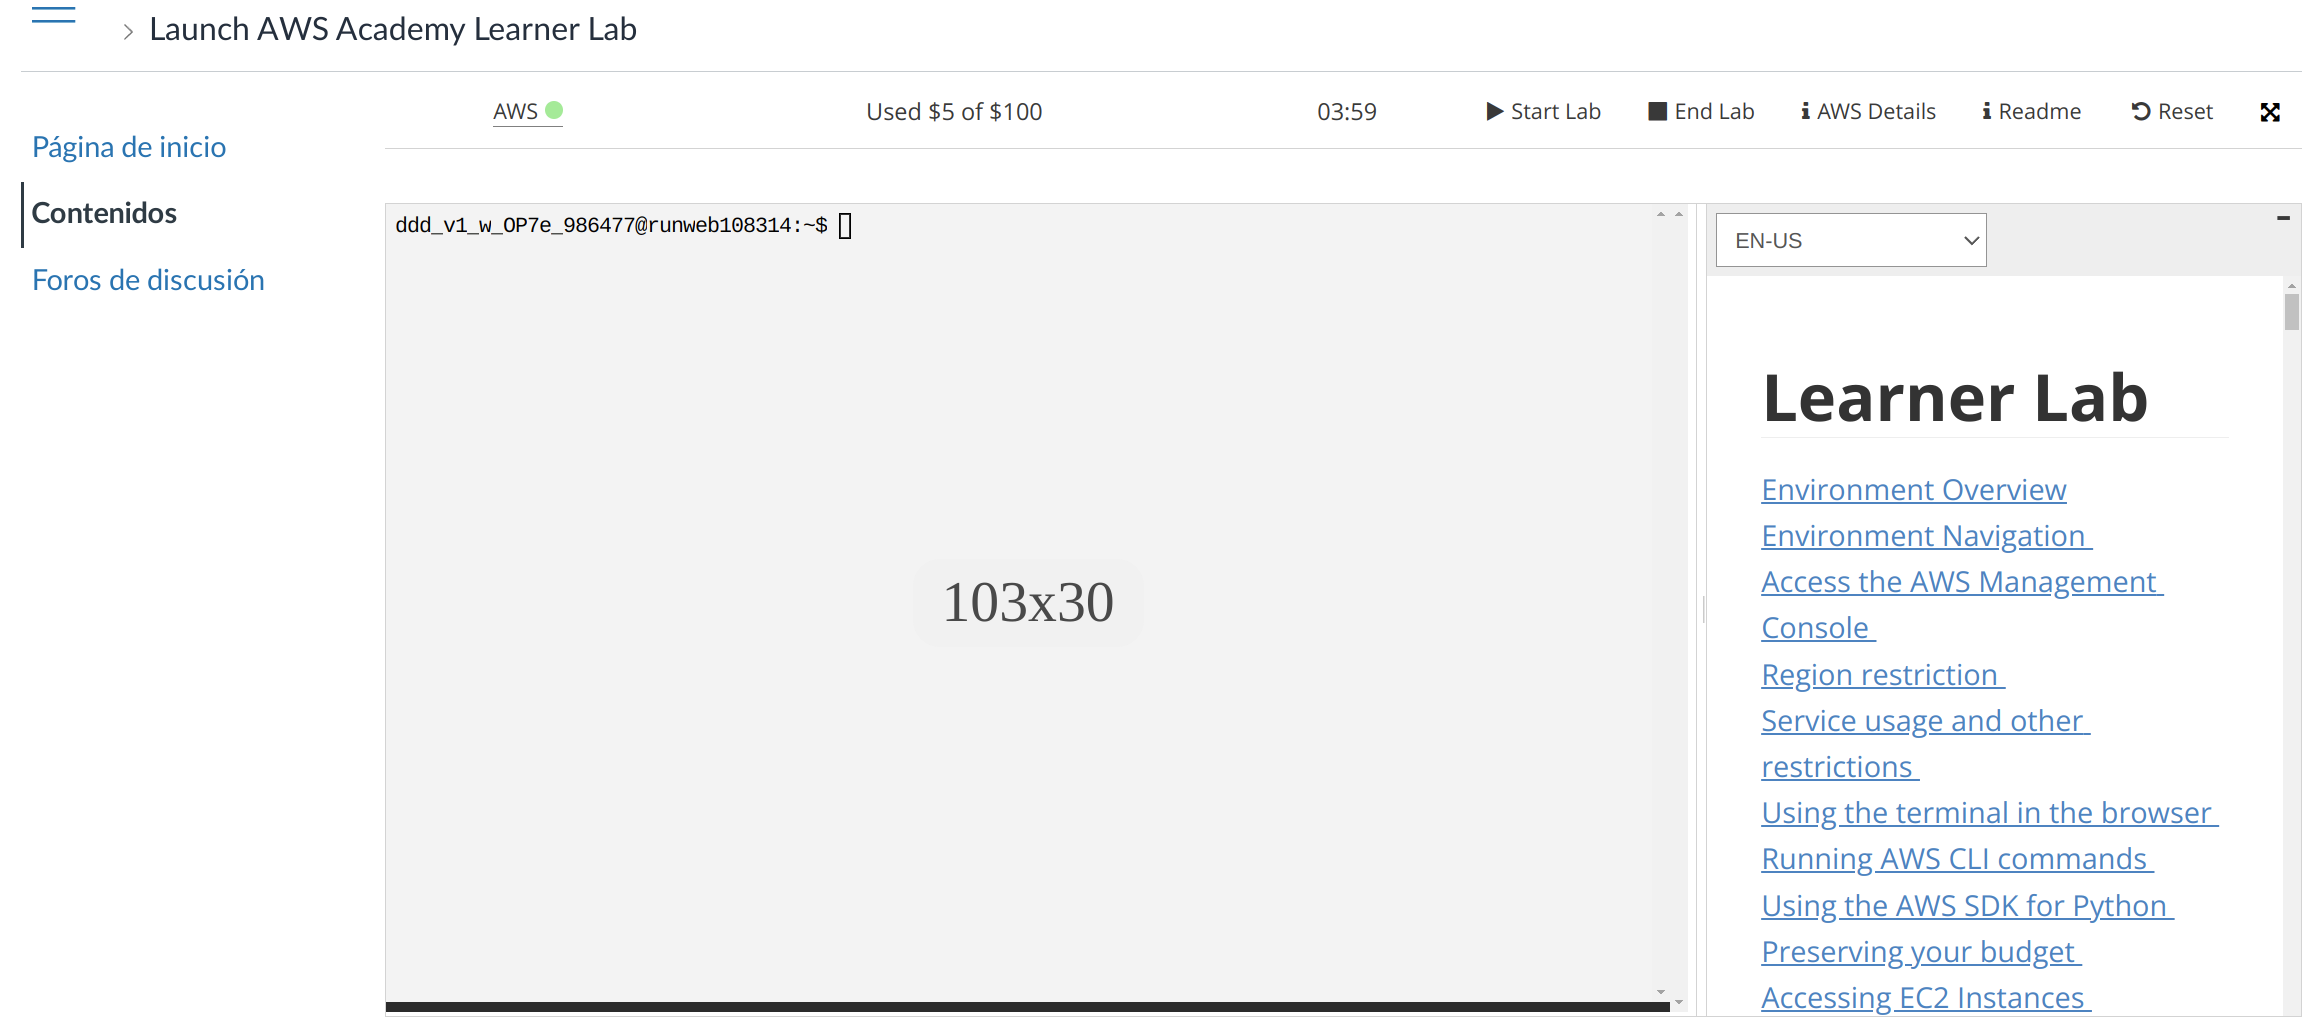
\includegraphics[frame, width=0.9\linewidth]{launcher-started.png}
\end{center}

Para entrar en el laboratorio debemos hacer click en “{AWS \color{green}●}”, lo que nos abrirá una nueva pestaña en la que veremos el panel de administración (o “Consola” llamada por AWS) donde tendremos un resumen de los servicios que hemos visitado anteriormente, aplicaciones que tengamos desplegadas, coste... La idea es tener a simple vista lo que más estemos utilizando.


\chapter{Servicios básico de AWS}

AWS cuenta hoy en día con infinidad de servicios que podemos utilizar y desplegar. Es imposible abarcar todos en un curso, por lo que aprenderemos a utilizar y a entender sólo de unos pocos. Entre los que vamos a utilizar están:

\begin{itemize}
	\item \textbf{VPC}: Es la parte que nos proporciona la red virtual en la nube de Amazon, y todo lo que tiene que ver con direccionamiento de red, acceso a internet, ... 
	\item \textbf{EC2}: Parte central de AWS que se encarga de la computación virtual y otros servicios que tienen que ver con máquinas virtuales.
	\item \textbf{RDS}: Es el servicio para crear bases de datos relacionales de Amazon. Podemos crear servicios con distintos motores, con distinta configuración, escalado, ...
\end{itemize}

Cuando entremos a algunos de estos servicios, el interfaz web que nos vamos a encontrar, por norma general, suele ser muy parecido y tiene el siguiente aspecto:

\begin{center}
	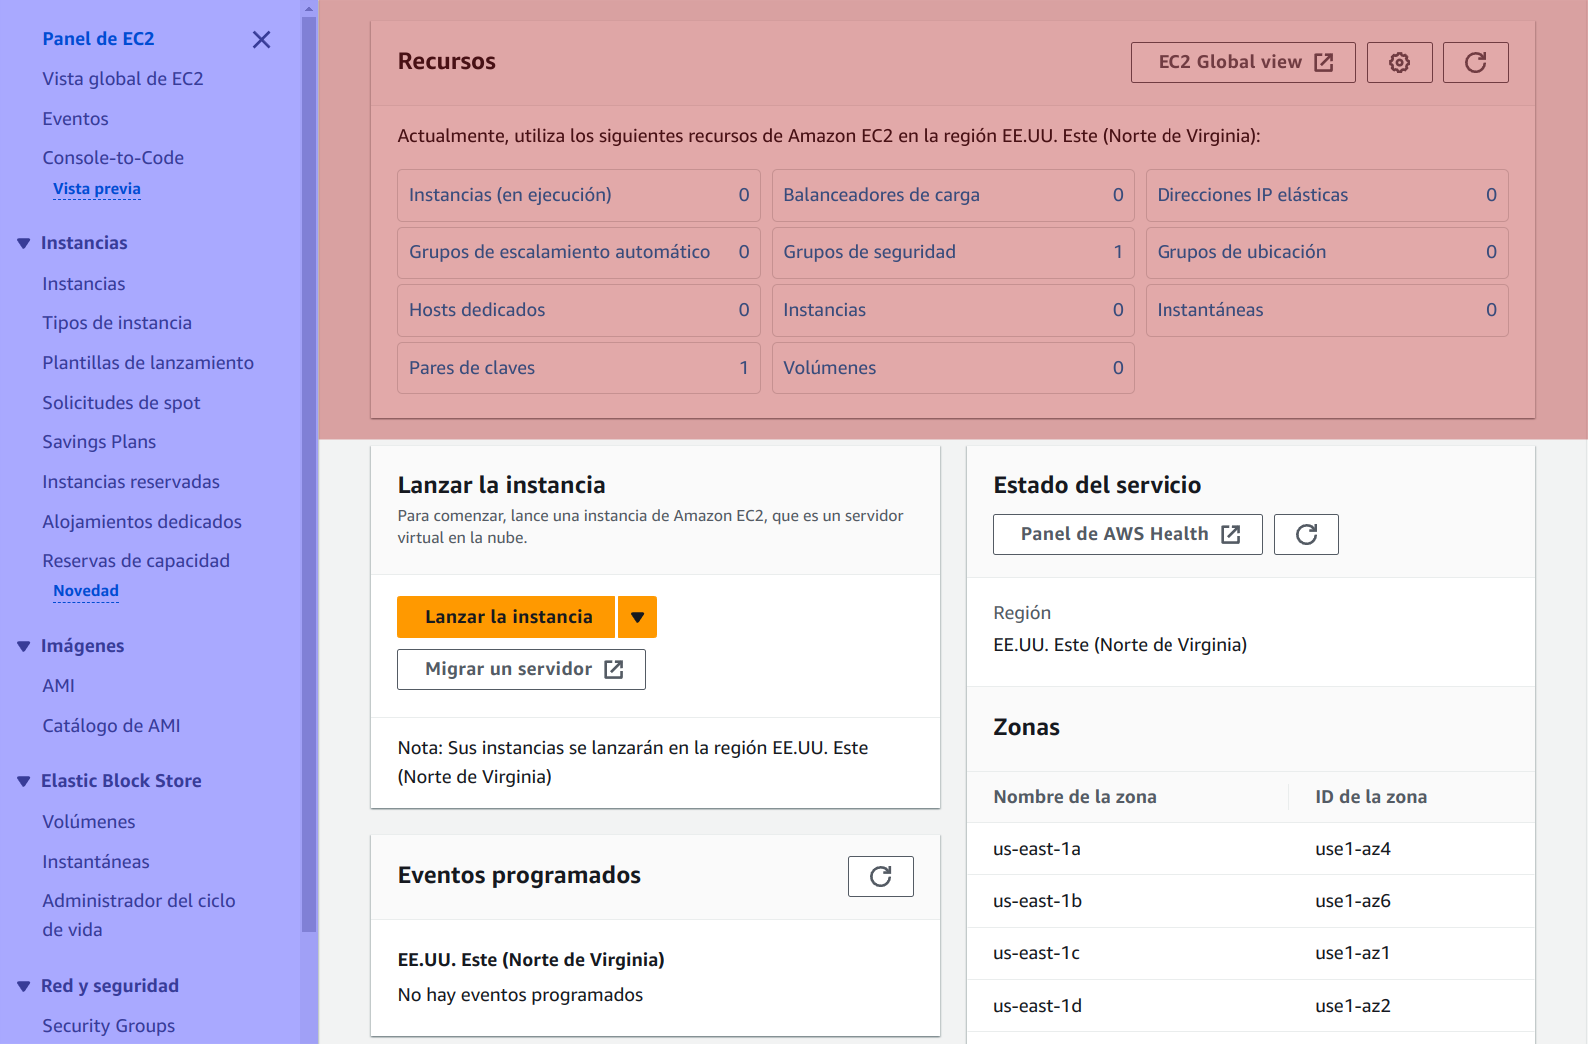
\includegraphics[width=0.8\linewidth]{panel.png}
\end{center}

Podemos diferenciar dos apartados en la vista:
\begin{itemize}
	\item \textbf{Panel lateral izquierdo}: En la imagen resaltado de color azul, es un menú donde podemos ver distintos apartados diferenciados por grupos. Estos apartados nos permitirán crear o configurar servicios que se nos desplegarán en la vista principal.
	
	\item \textbf{Vista principal}: En este caso sólo se ha resaltado la parte superior, ya que al entrar a cada tipo de servicio, en esta parte aparece un resumen de los recursos que tenemos contratados.
	
	Esta vista central cambiará teniendo en cuenta la opción seleccionada del panel lateral.
\end{itemize}

\chapter{Regiones y zonas de disponibilidad}

Dado que AWS ofrece un servicio mundial, los servidores que nos ofrecen están desplegados a lo largo de distintos países, para que el acceso desde cada zona sea lo más rápida posible. Esta infraestructura global, actualmente está diferenciada de la siguiente manera tal como aparece en la \href{https://aws.amazon.com/es/about-aws/global-infrastructure/regions_az/?p=ngi&loc=2}{documentación oficial}:

\begin{center}
	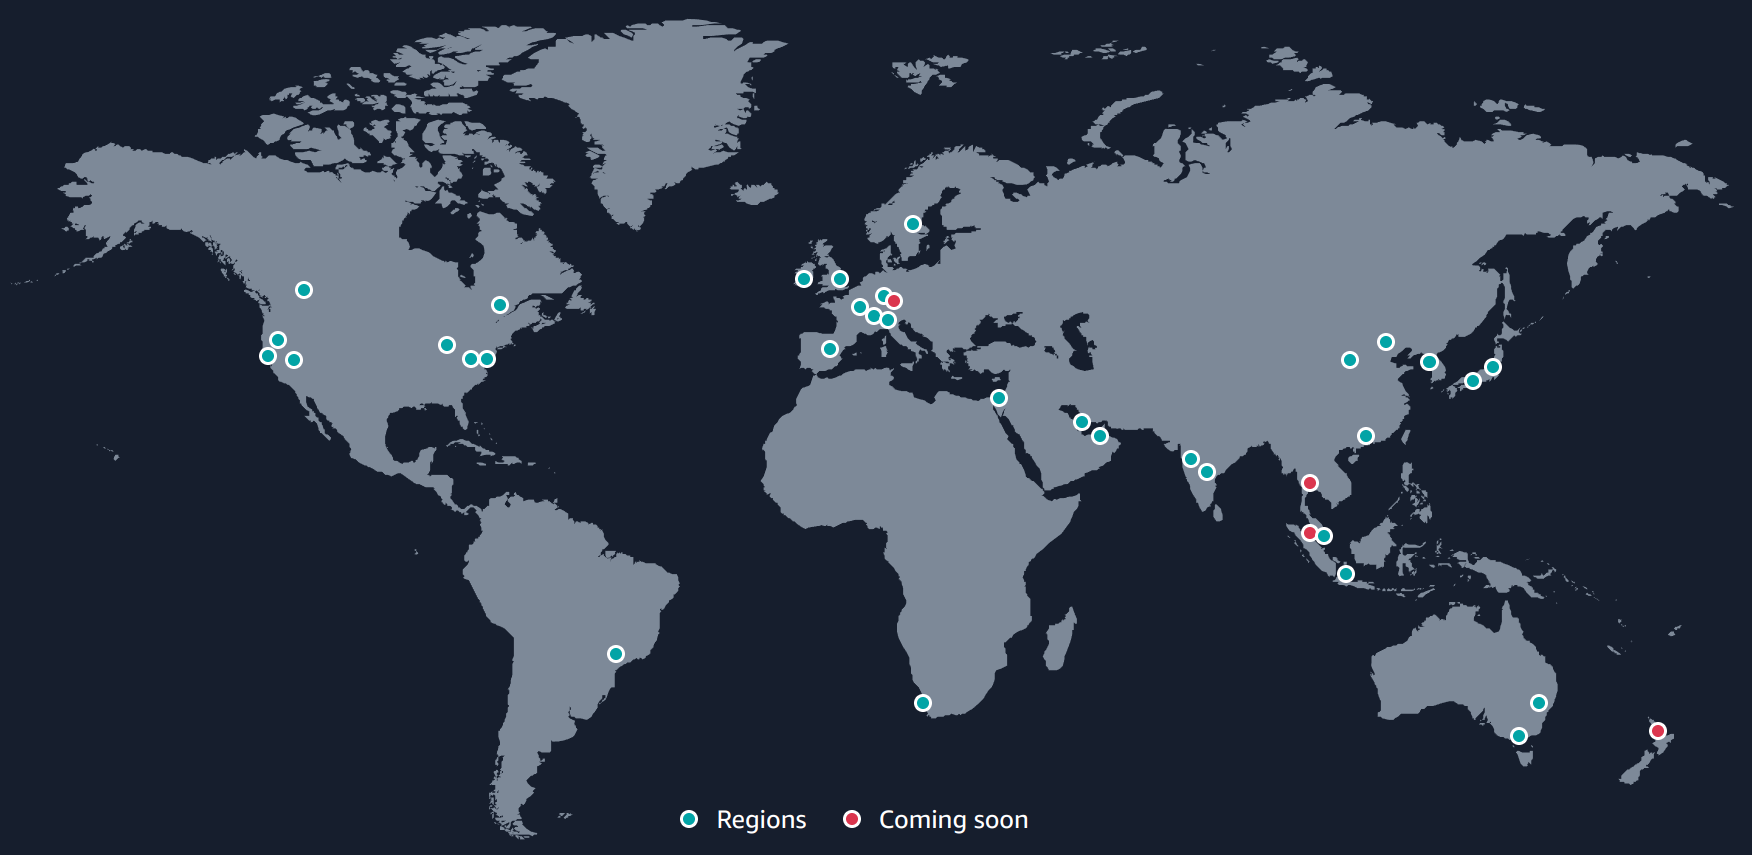
\includegraphics[width=0.8\linewidth]{regiones.png}
\end{center}

\begin{itemize}
	\item \textbf{Regiones}: AWS tiene el concepto de una región, que es una ubicación física en todo el mundo donde se agrupan los centros de datos. Se llama a cada grupo de centros de datos lógicos “zona de disponibilidad”. 
	
	Ejemplo de Regiones en Europa: España (situada en Aragón), Irlanda, Fráncfort, Londres, París, Estocolmo, Milán, Zúrich.
	
	\item \textbf{Zonas de disponibildiad}: Cada región de AWS consta de un mínimo de tres zonas de disponibilidad con acceso aisladas y físicamente separadas dentro de un área geográfica. 
	
	El diseño múltiple de zonas de disponibilidad de cada región de AWS ofrece ventajas para los clientes. Cada zona de disponibilidad tiene alimentación, refrigeración y seguridad física independientes y está conectada a través de redes redundantes de latencia ultrabaja.
	
	
\end{itemize}

\warnbox{\textbf{AWS Academy está limitado sólo a la región “Norte de Virginia” de Estados Unidos.}}

Por limitaciones de AWS Academy, todo lo que creemos sólo va a ser creado en la regiónd “Norte de Virginia” de Estados Unidos. Esto puede hacer que haya algo más de latencia desde España, pero el resultado de aprendizaje será el mismo.
    
    \part{Introducción a VPC}
    \chapter{Introducción}

VPC, por sus siglas en inglés \textit{Virtual Private Cloud}, es la infraestructura de red privada virtual  que se va a crear en la nube de AWS para nosotros, donde se podrán crear los servicios y añadir los recursos que posteriormente vamos a ver.

Podemos tener distintas redes virtuales VPC distintas, y en cada una de ellas alojar los servicios que nos interesen. De esta manera, podemos diferenciar proyectos o clientes, a través de distintos VPC, ya que cada uno de ellos está separado completamente del resto.

Aunque no vamos a realizar modificaciones al VPC creado por defecto en el laboratorio, es interesante conocer qué características existen y las posibilidades que podemos tener.

\chapter{Características}

El VPC creado en nuestro laboratorio cuenta con un direccionamiento privado con la red \textbf{172.31.0.0/16} que está situado en la zona de disponibilidad "\textbf{us-east-1}" (Norte de Virginia de Estados Unidos, tal como se ha dicho previamente). Una de las limitaciones de AWS Academy es que no podremos crear un VPC en otra zona de disponibilidad.

\infobox{\textbf{En una cuenta AWS normal se pueden crear VPC en distintas zonas geográficas.}}

Aunque no vamos a profundizar, conviene entender distintas características que nos podemos encontrar y que podemos contratar o modificar.

\errorbox{\textbf{El apartado VPC puede ser uno de los más complejos de entender dentro de todo AWS. Es por eso que no vamos a profundizar en ello.}}

\section{Subredes, tablas enrutamiento y acceso a internet}

Para entender y modificar este apartado hay que tener conocimientos profundos de redes, por lo que hay que tenerlo en cuenta si se decide realizar algún tipo de modificación en estos apartados.

\begin{itemize}
	\item \textbf{Subredes}: El VPC que tenemos por defecto consta de distintas subredes, cada una de ellas creada en una zona de disponibilidad diferente dentro de la región. Esto permite la alta disponibilidad de nuestros servicios.
	
	\item \textbf{Enrutamiento}: Básicamente nos indica qué se debe hacer con las rutas dentro de la red. Como de la red local de casa, tenemos dos apartados:
	\begin{itemize}
		\item \textbf{La propia red}: Es decir, el direccionamiento del propio VPC, 172.31.0.0/16. Es como si fuese la red de casa.
		
		\item \textbf{0.0.0.0}: Es el resto de direcciones que no coinciden con la red local, y que lo que hará con ellas será redirigirlas al “\textit{internet gateway}”. Sucede lo mismo en nuestra casa, que las direcciones que no son la propia red se mandan al router.
	\end{itemize}
	
	\item \textbf{Internet \textit{gateway}}: Es el sistema que permite la conexión entre el VPC e internet.
\end{itemize}

\errorbox{\textbf{No vamos a realizar ninguna modificación de la configuración que tenemos por defecto.}}


    \part{Introducción a EC2}
    \chapter{Introducción}

\textbf{EC2}, contracción de las siglas en inglés \textit{Elastic Compute Cloud}, es la parte central de AWS que tiene que ver con la computación, donde podremos crear máquinas virtuales y gestionar todo lo relacionado con ellas.

Dentro del apartado EC2 podremos crear las máquinas virtuales (llamadas \textbf{instancias}) donde después alojaremos o desplegaremos los servicios que nos interese. También podremos crear backups de ellas, crear imágenes para levantar instancias de manera más rápida, securizarlas...

\chapter{Instancias}

Una instancia es cómo llama AWS a una máquina virtual, por lo que los conocimientos previos que tengamos sobre máquinas virtuales se pueden asociar una instancia EC2 de AWS. Podemos realizar distintas acciones sobre las instancias que ya tengamos creadas.

Antes de crear una instancia debemos entender distintos apartados ya que a la hora de lanzar una instancia (crearla), se nos pedirá que elijamos entre distintas opciones disponibles. Es similar a lo que sucede cuando creamos una máquina virtual con Virtualbox.

\section{Tipos de instancia}

El tipo de instancia hace referencia a parte del hardware que va a tener disponible la máquina virtual al realizar el despliegue. Existe una infinidad de tipos de instancias, y es por eso que conviene leer la \href{https://docs.aws.amazon.com/AWSEC2/latest/UserGuide/instance-types.html#AvailableInstanceTypes}{documentación oficial} ya que en ella se detalla mucho más para qué sirve cada una de ellas.

Los nombres de las instancias siguen un convenio que viene explicado en la documentación oficial.

\begin{center}
	\includesvg[]{ec2_instance_name_convention.svg}
\end{center}

Dado que el número de tipos de instancias actualmente es mayor que 700, puede resultar complejo saber exáctamente de primera mano cuál debemos elegir. Por otro lado, en el listado que podemos ver en el panel de EC2, nos aparece la información que a simple vista nos puede dar una idea de cómo es el tipo de instancia.

\infobox{\textbf{Para asegurar que se adecúa a nuestras necesidades, es mejor confirmar el tipo de instancia que necesitamos mirando la \href{https://docs.aws.amazon.com/AWSEC2/latest/UserGuide/instance-types.html}{documentación oficial}.}}

\begin{center}
	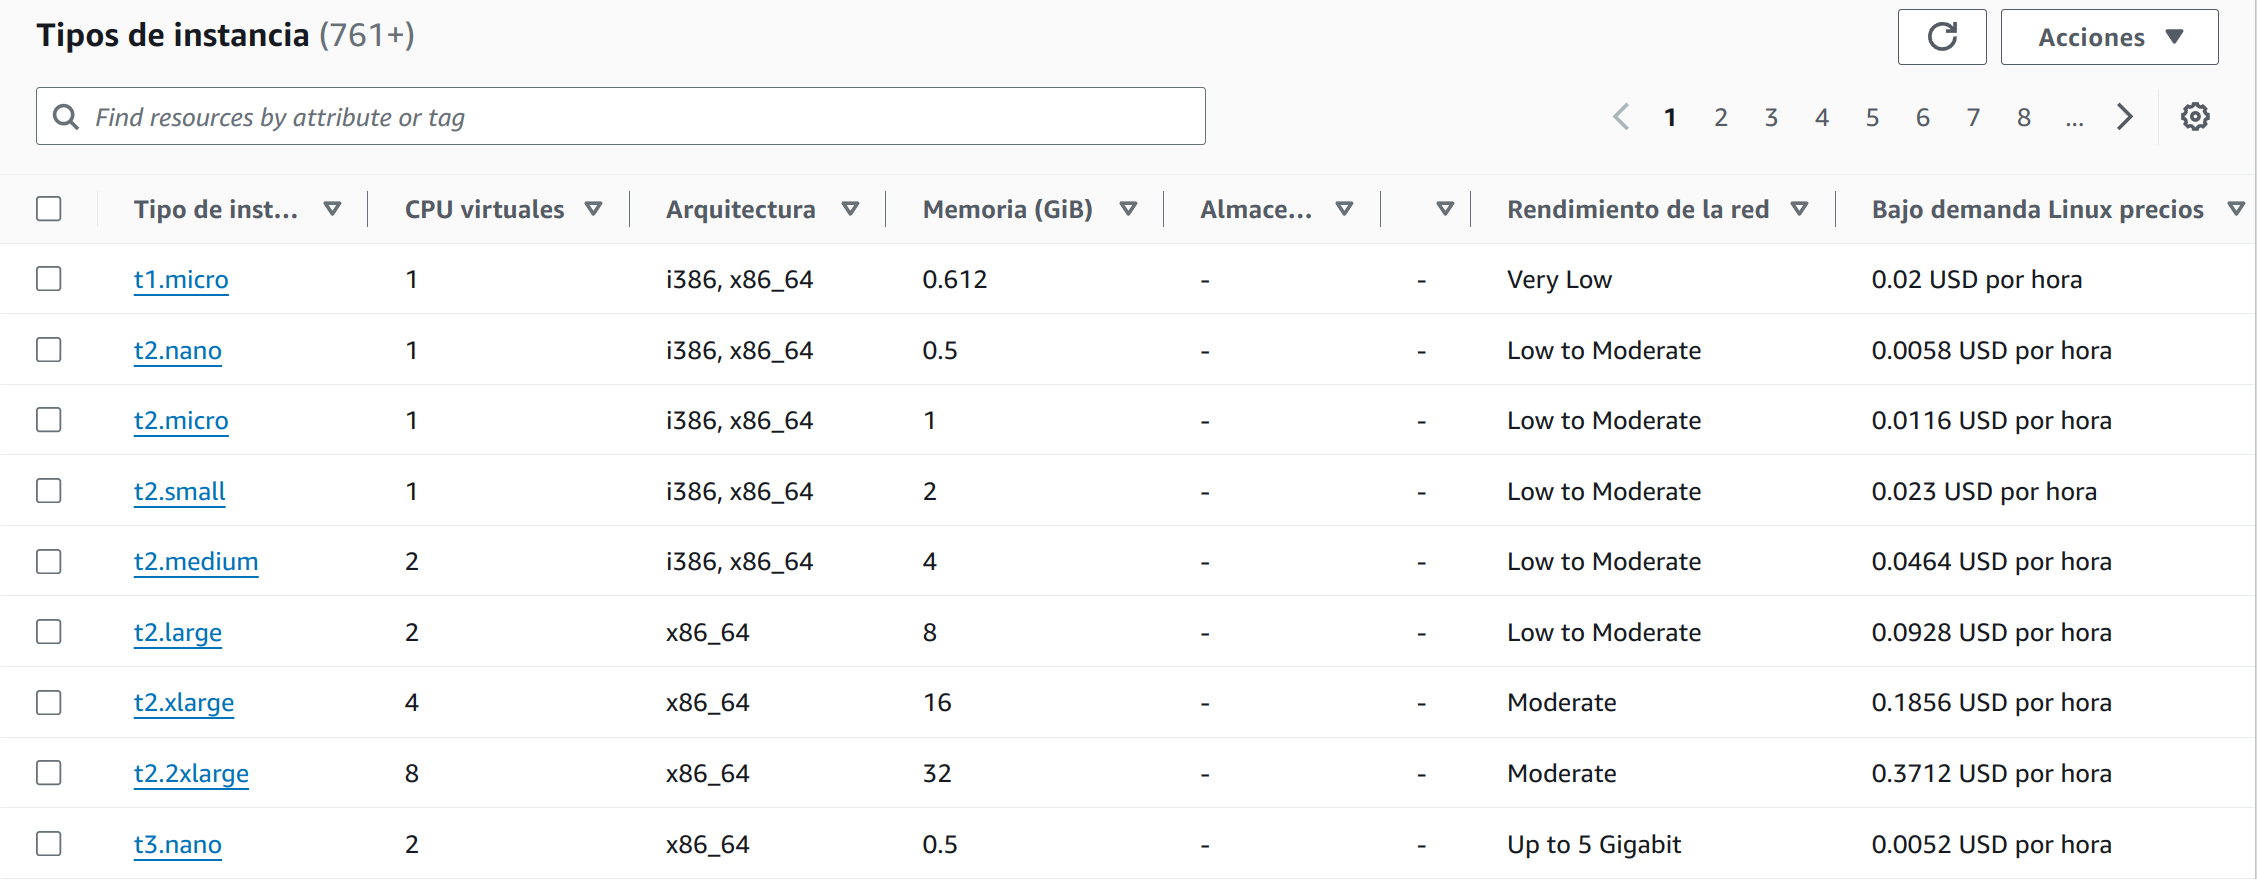
\includegraphics[frame,width=0.9\linewidth]{ec2_instance_types.png}
\end{center}

Los valores que podemos identificar a simple vista son:

\begin{itemize}
	\item \textbf{CPU virtuales}: El número de cores virtuales que el procesador virtual tendrá a su disposición. Dependiendo de nuestras necesidades de cómputo y procesamiento, deberemos elegir un número que se adecúe al rendimiento que esperamos. Actualmente podemos elegir tipos de instancias que tengan entre 1 y 448 CPUs.
	
	\item \textbf{Arquitectura}: Es el tipo de arquitectura del procesador con el que se desplegará la máquina virtual. Entre las arquitecturas que podemos elegir están:
	\begin{itemize}
		\item \textbf{i386}: Arquitectura clásica de equipos de 32 bits.
		\item \textbf{x86\_64}: Arquitectura actual para equipos y servidores.
		\item \textbf{x86\_64\_mac}: Arquitectura utilizada por los equipos Mac con procesadores Intel.
		\item \textbf{arm64}: Arquitectura ARM de 64 bits.
		\item \textbf{arm64\_mac}: Arquitectura ARM de los nuevos procesadores M* de Apple.
	\end{itemize}
	
	\item \textbf{Memoria}: Tamaño de la memoria RAM medido en GiB.
	
	\item \textbf{Rendimiento de la red}: Velocidad de la conexión de red que tendrá la instancia.
	
	\item \textbf{Precio de la instancia}: El coste de la instancia cuando está en funcionamiento se mide en doláres americanos (USD) por hora. El precio varía si el sistema operativo que va a correr la instancia es Linux o Windows, y por supuesto del resto de componentes virtuales.
	
\end{itemize}

\warnbox{\textbf{Se puede cambiar el tipo de instancia, pero para ello se debe parar la instancia}. }


\section{Imágenes AMI}

Una imagen AMI (\textit{Amazon Machine Image})es una plantilla que contiene la configuración del software (el sistema operativo, los servicios y aplicaciones) que son necesarias para correr dentro de nuestra instancia. Existen imágenes AMI públicas creadas por proveedores de software verificados entre las que podremos elegir. 

Hay un catálogo de AMI entre las que podemos elegir:

\begin{itemize}
	\item \textbf{Quickstart AMIs}: Imágenes que normalmente suelen ser el sistema operativo con el mínimo software necesario para hacerlo funcionar. Para correr el resto de servicios, necesitaremos instalar lo que necesitemos.
	
	\item \textbf{Mis AMI}: Podemos crear nuestras propias imágenes para poder reusarlas cuando queramos.
	
	\item \textbf{AMI de AWS Marketplace}: Son imágenes creadas por empresas que pueden contener servicios de alto rendimiento, y \textbf{que en muchos casos pueden ser de pago (por licencia o uso)}.
	
	\item \textbf{AMI de la comunidad}: Imágenes que pueden ser creadas por proveedores oficiales o por comunidades que crean imágenes con software específico.
\end{itemize}

\begin{center}
	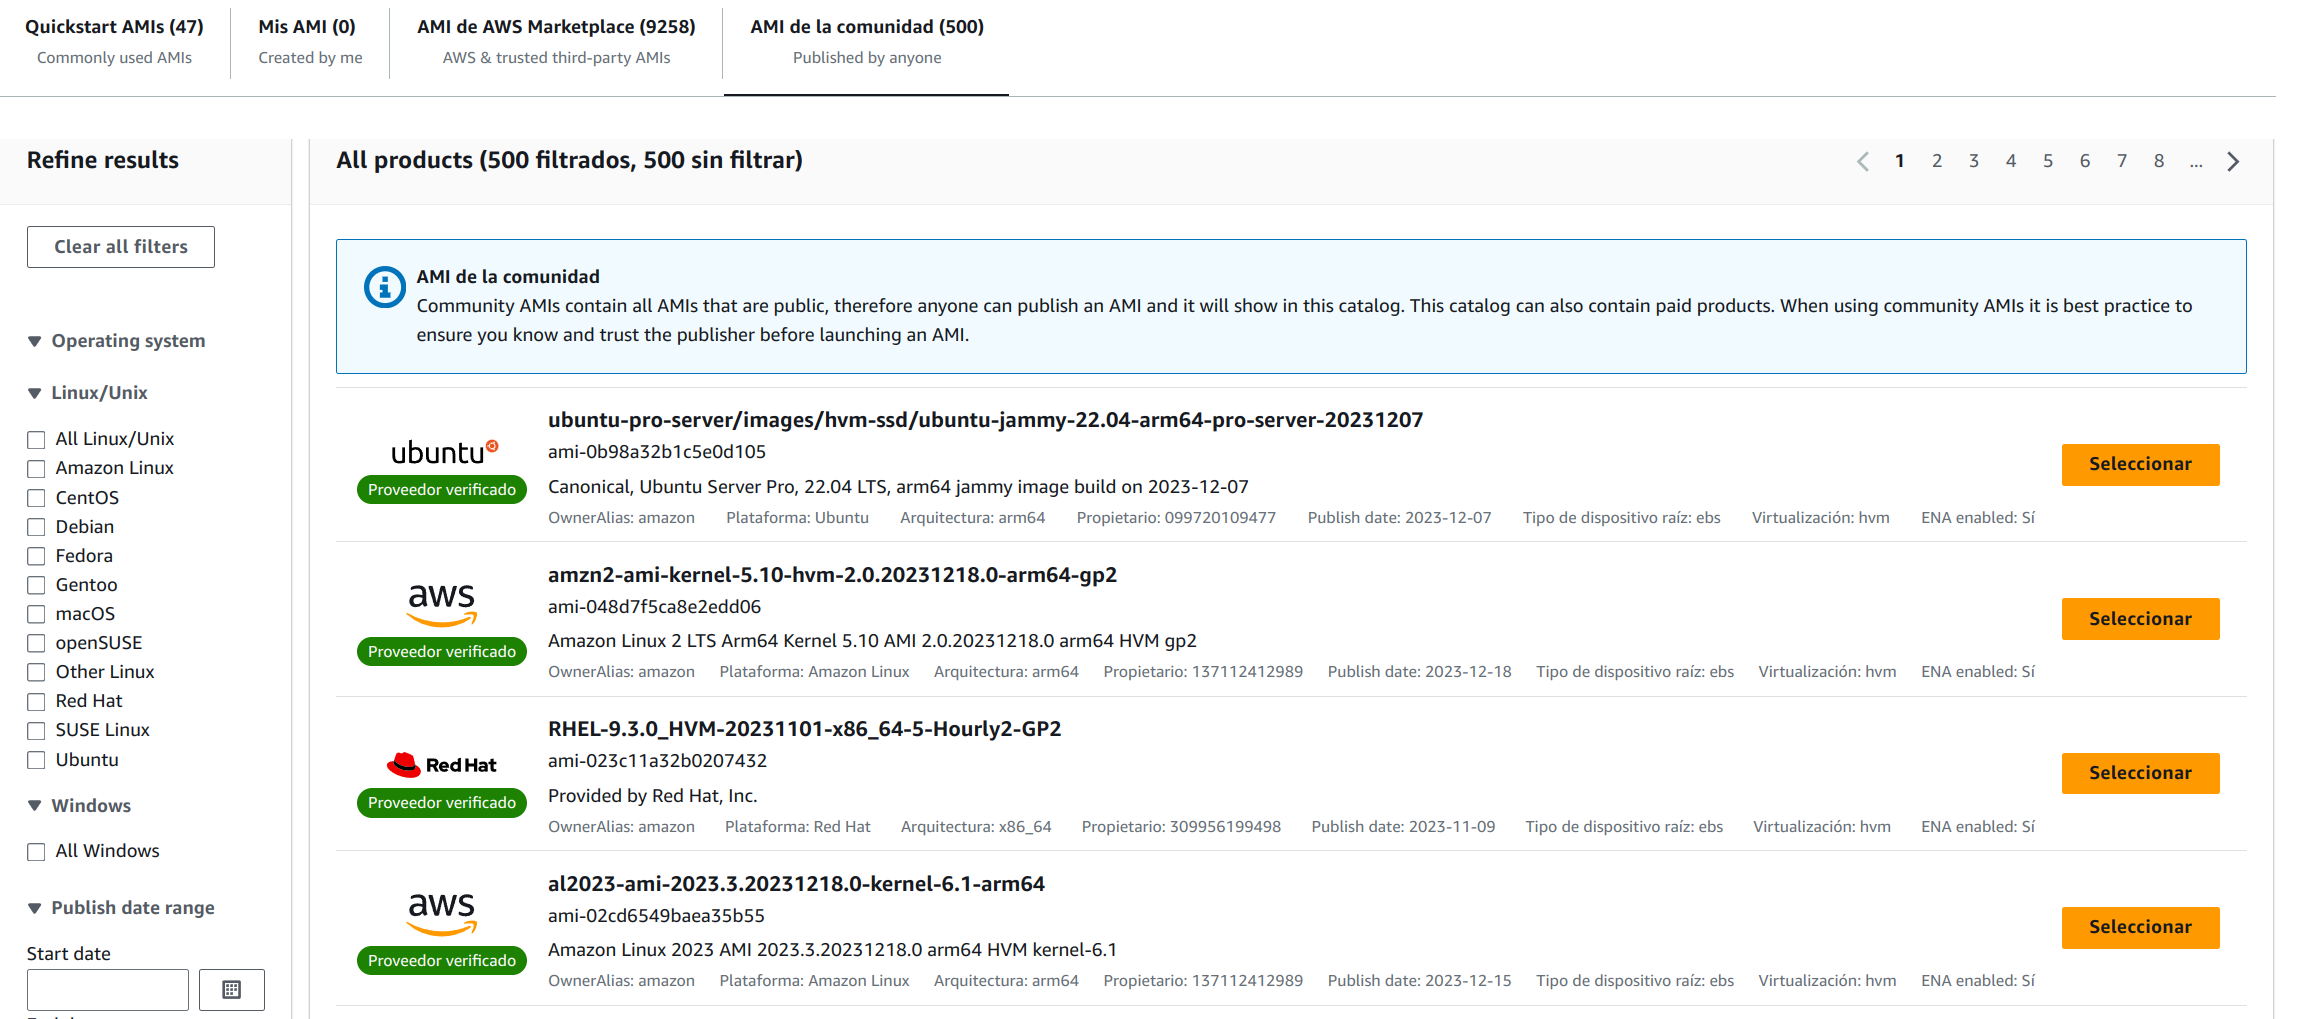
\includegraphics[frame,width=\linewidth]{ec2_ami_catalogue.png}
\end{center}




\infobox{\textbf{Podemos crear nuestras propias imágenes para poder reusarlas cuando queramos.}}

Para empezar, podemos crear nuestra instancia con una imagen AMI de un proveedor oficial, para posteriormente utilizarla como base para crear una AMI propia.


\section{Crear una instancia}

A continuación se va a explicar cómo crear una instancia de tipo Linux teniendo en cuenta todas las posibles opciones que podemos elegir. Para crearla haremos click en 
\includegraphics[height=0.8\baselineskip]{ec2_instance_create.png} y seguiremos las indicaciones para adecuarla a nuestras necesidades.

Las respuestas que debemos contestar y tener en cuenta son:

\begin{itemize}
	\item \textbf{Nombre y etiquetas}: Es el nombre que le vamos a dar a la instancia (que debería ser un nombre significativo), y posibles etiquetas para identificarla.
	
	\item \textbf{Application and OS Images (Amazon Machine Image)}: Imagen AMI que queremos desplegar en la instancia.
	
	\item \textbf{Arquitectura}: Arquitectura del procesador.
	
	\item \textbf{Tipo de instancia}: El tipo de instancia que queremos desplegar para las necesidades que tenemos.
	
	\item \textbf{Par de claves (inicio de sesión)}: El par de claves asimétricas (\textbf{pública-privada}) que vamos a utilizar para realizar la conexión a la instancia. Más adelante explicaremos cómo acceder a la instancia. 
	
	\warnbox{\textbf{Debemos elegir el par de claves “vockey” para poder acceder a la instancia.}}
	
	\item \textbf{Configuraciones de red}: Ajustar las configuraciones de red. Por defecto podemos elegir el \textbf{grupo de seguridad} que queremos asignar a la instancia. Como opciones avanzadas, podemos desactivar el tener IP pública o asignar la instancia a una subred.

	\errorbox{\textbf{La IP pública que se asigna no es “eterna”. Cuando se apague la instancia y se vuelva a levantar obtendrá otra IP pública.}}
	
	\item \textbf{Configurar almacenamiento}: El disco duro principal de la instancia.
	
	\item \textbf{Opciones avanzadas}: Distintas opciones de configuraciones que podemos modificar o de hardware que podemos habilitar.
\end{itemize}

A la derecha del asistente tenemos tenemos un resumen en el que nos aparece las distintas opciones seleccionadas. En este resumen podemos elegir el número de instancias que nos interese crear, por si queremos más de una.

Una vez le damos a “Lanzar instancia” la instancia se creará y empezará el despliegue. Desde el panel de instancias, si seleccionamos la instancia recién creada veremos todos los detalles de la misma:

\begin{center}
	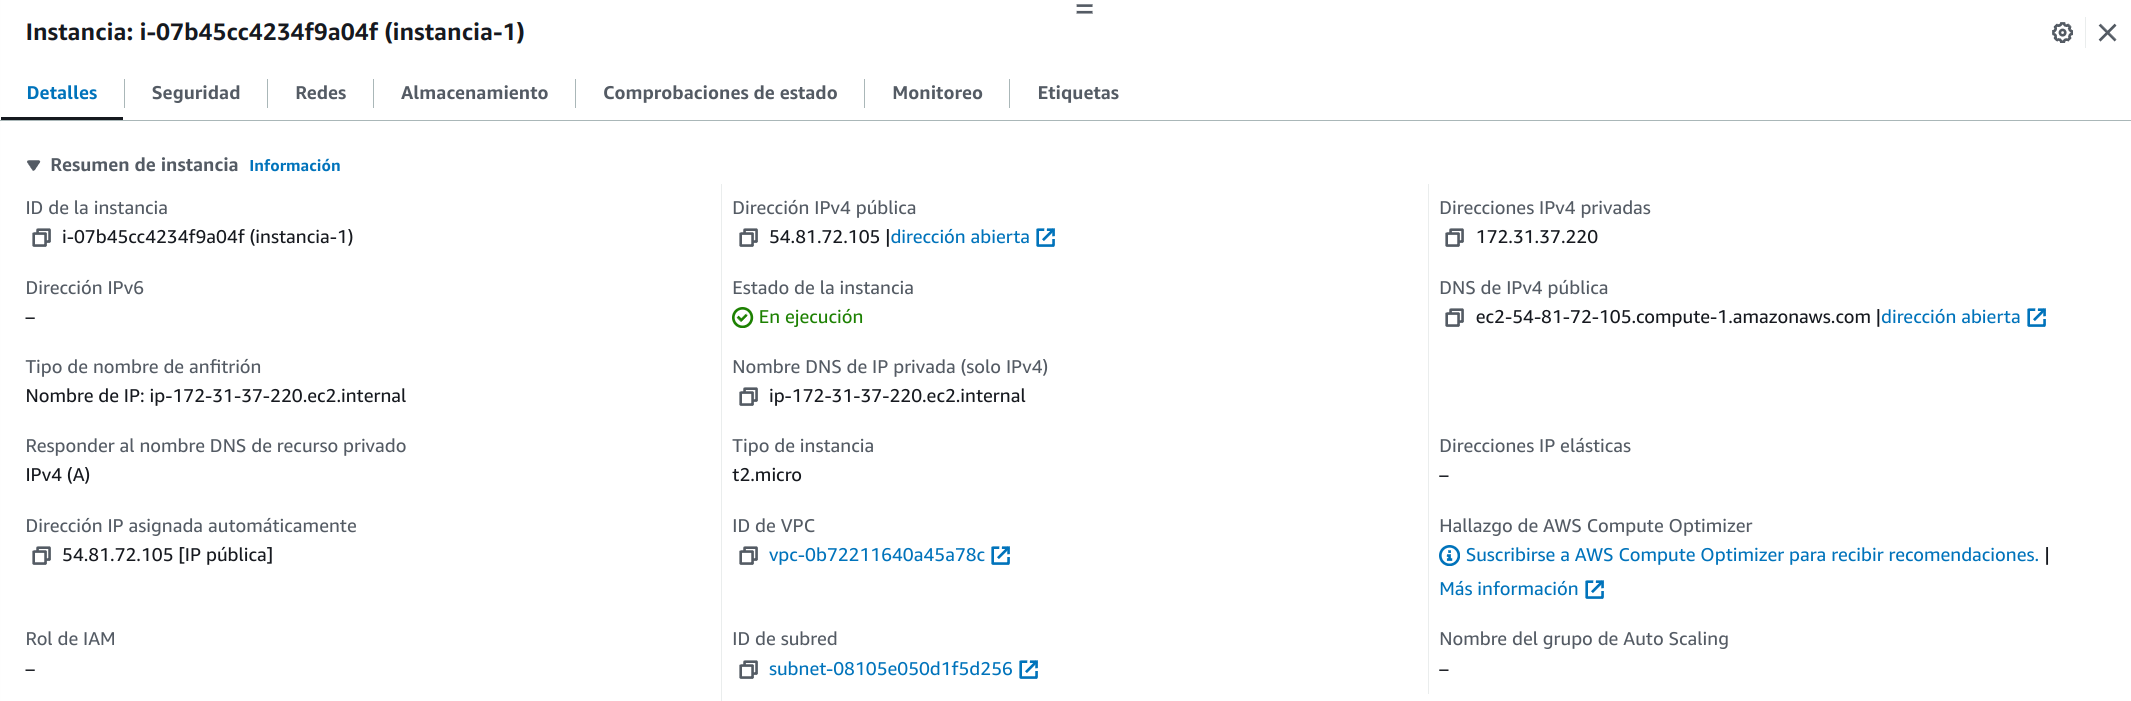
\includegraphics[frame,width=0.9\linewidth]{ec2_instance_info.png}
\end{center}

Tal como se puede ver, la información de la instancia está separada en distintas pestañas y en cada una de ellas nos aparecerá mucha información sobre la misma. Parte de esta información será la necesaria para poder acceder a la instancia por SSH.


\section{Acceder a una instancia}

Para acceder a una instancia desplegada tenemos distintas opciones que podemos visualizar desde el botón 
\includegraphics[height=0.8\baselineskip]{ec2_instance_connect.png} cuando esté la instancia seleccionada. Entre las opciones, vamos a destacar dos:

\begin{itemize}
	\item \textbf{Conexión de la instancia EC2}: Es el método más sencillo para acceder a una instancia a través de SSH, ya que vamos a poder realizar la conexión a través del propio navegador web. Esto, por otro lado, no nos va a permitir hacer uso de todas las características que tiene una terminal real.
	
	\item \textbf{Cliente SSH}: Al igual que sucede al conectarnos a una máquina virtual normal,  podemos acceder a la instancia a través de un cliente SSH de consola. Para ello, necesitamos conocer:
	\begin{itemize}
		\item \textbf{Nombre de usuario}: Dependiendo de la AMI que hayamos desplegado, el usuario de conexión será distinto. Por ejemplo, para instancias Ubuntu el usuario es “\textbf{ubuntu}”; para instancias Debian el usuario es “\textbf{admin}”; para instancias Amazon Linux, el usuario es “\textbf{ec2-user}”. \textbf{Estos usuarios tienen la posibilidad de convertirse en “root” usando el comando “sudo”}.

		\infobox{\textbf{Dependiendo de la AMI elegida, el usuario de acceso será distinto.}}

		\item \textbf{DNS público / IP pública}: Lógicamente, para poder acceder a la instancia, debemos conocer cuál es su IP pública. También se puede hacer uso del DNS público, que está asociado a la IP, pero de nuevo, este cambia.
		
		\errorbox{\textbf{La IP pública que se asigna no es “eterna”. Cuando se apague la instancia y se vuelva a levantar obtendrá otra IP pública.}}
		
		\item \textbf{Clave privada de acceso}: El usuario por defecto de la instancia no cuenta con contraseña, por lo que para acceder necesitamos hacer uso de una autenticación basada en \textbf{clave asimétrica} (conocidas también como “\textbf{clave pública-privada}”).
		
		\warnbox{\textbf{Para poder acceder a la instancia es necesario usar claves asimétricas.}}
		
	\end{itemize}
\end{itemize}


\subsection{Obtener clave privada}

Tal como se ha dicho previamente, para poder acceder a las instancias recién creadas debemos hacer uso del sistema de claves asimétricas, ya que es el método más seguro de conexión, y así no dependemos de contraseñas.

Al crear el laboratorio se nos ha creado un par de claves llamadas “\textbf{vockey}”, que sólo podemos descargar desde el panel del curso, en el apartado “\faInfo  \textbf{ AWS Details}”, dándole al botón 
\includegraphics[height=0.8\baselineskip]{ec2_download_pem.png}, que nos descargará un fichero llamado \textbf{labuser.pem}.

\textbf{Este fichero de clave debe tener permisos especiales}. Los ficheros de tipo Linux son que sólo debe tener permisos de lectura para el usuario, dejando el resto de permisos sin asignar. Por lo tanto, en formato binario, \textbf{400}. Para ello debemos hacer:

\begin{mycode}{Cambios de permisos en el fichero}{console}{}
ruben@vega:~$ chmod 400 labuser.pem
\end{mycode}

Para realizar la conexión a la instancia, y teniendo en cuenta los datos comentados previamente, el acceso se realizará utilizando el siguiente comando, sustituyendo los datos por los correspondientes para la instancia:

\begin{mycode}{Conexión a una instancia mediante cliente SSH}{console}{}
ruben@vega:~$ ssh -i labsuser.pem admin@52.91.155.75 
admin@ip-172-31-32-168:~$ sudo su
root@ip-172-31-32-168:/home/admin#
\end{mycode}

De esta manera, ya estaremos dentro de la instancia desplegada en AWS, y podremos empezar a desplegar el servicio que nos interese.


\subsection{Crear nuevo par de claves}
En entornos profesionales \textbf{es habitual crear distintas par de claves para cada proyecto, o incluso para cada instancia}, ya que de conseguir una (o en sistemas basados en contraseñas), se obtendría acceso a un gran número de instancias, \textbf{lo que es un fallo de seguridad de extrema gravedad}.

\errorbox{\textbf{En entornos profesionales nunca se debería reutilizar claves, y menos entre distintos proyectos.}}

Si queremos crear un nuevo par de claves lo podemos realizar desde el menú lateal, en el apartado: “\textbf{Red y seguridad → Pares de claves}”. Ahí podremos hacer click sobre el icono 
\includegraphics[height=0.8\baselineskip]{ec2_new_key.png}, que nos redirigirá a un formulario donde crear las nuevas claves.

\begin{center}
	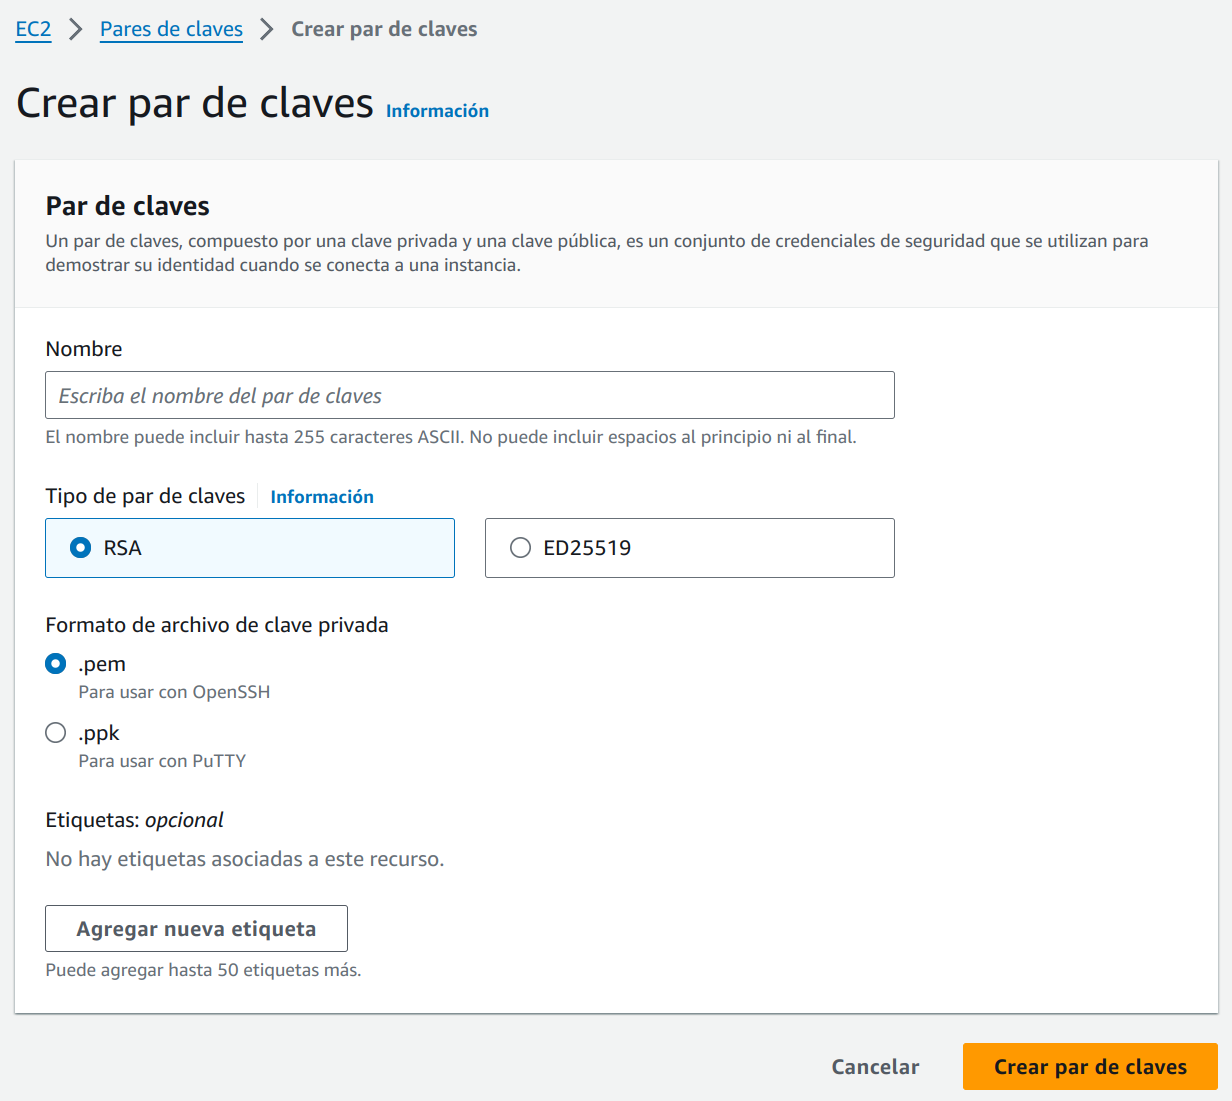
\includegraphics[frame,width=0.9\linewidth]{ec2_new_key2.png}
\end{center}

Una vez rellenado los datos, al darle al botón de crear, se nos descargará el fichero \textbf{que nunca más podremos volver a descargar}, por lo que deberemos guardarla a buen recaudo. A partir de ahora, al crear una nueva instancia, podremos hacer uso de esta nueva clave para el poder realizar el acceso con ella.

\errorbox{\textbf{¡Cuidado con el certificado descargado! No lo podremos volver a descargar.}}


\chapter{Direcciones IP elásticas}

Una IP elástica es una \textbf{IPv4 de direccionamiento público} que podemos asignar a una instancia EC2 (o a un interfaz de red de una EC2) que hayamos creado. Esta dirección IP estará asociado a nuestro VPC aunque la instancia EC2 no esté en funcionamiento.

\warnbox{\textbf{Las direcciones IP elásticas se cobran aparte. Es mejor no contratar una IP elástica hasta que el servicio no se vaya a poner en producción.}}

Las instancias EC2 no cuentan siempre con la misma IP pública, y es por eso que si queremos que nuestro servicio públicamente siempre tenga la misma IP debemos asociarle una IP elástica.


\chapter{Security Groups}

Los grupos de seguridad, o \textbf{\textit{security groups}}, actúan como un \textbf{firewall} virtual que controla el tráfico de una o varias instancias. Al crear una instancia se puede especificar uno o varios grupos de seguridad, o se pueden añadir más adelante. Por defecto, \textbf{con cada instancia se nos creará un security group nuevo}.

Lo ideal es crear security groups que se reutilicen entre varias instancias, ya que si después modificamos las reglas de este security group, se aplicará a todas las instancias a las que esté asignado. Los security group cuentan con \textbf{reglas de entrada y de salida}.

\section{Crear security group}

Los security group se pueden crear desde el panel de \textbf{VPC} o de \textbf{EC2}. En este último caso dentro del apartado “\textbf{Red y seguridad → Security Groups}” y dándole al botón 
\includegraphics[height=0.8\baselineskip]{ec2_security_group_create.png}, que nos llevará a un formulario donde podemos rellenar:

\begin{itemize}
	\item Nombre del grupo de seguridad
	\item Descripción
	\item VPC al que pertenece
	\item Reglas de entrada
	\item Reglas de salida
\end{itemize}

\section{Reglas de entrada}

Tal como hemos dicho, un security group es un \textbf{firewall}, por lo que \textbf{si no tenemos reglas de entrada, por defecto todo el tráfico estará bloqueado}. Esta es la manera más segura para que no haya ninguna conexión no controlada que llegue a la instancia.

\infobox{\textbf{Las reglas de entrada son el tráfico que queremos permitir entrar a la instancia.}}

A la hora de crear una regla de entrada, \textbf{que será el tráfico que queremos permitir}, tendremos que elegir entre:

\begin{itemize}
	\item \textbf{Tipo de regla}: Nos aparece un menú desplegable en el que podremos elegir entre distintos tipos de reglas ya creadas. Dependiendo de la regla seleccionada, no nos permitirá elegir ni protocolo ni puertos, ya que por defecto los habrá rellenado la regla elegida.
	\item \textbf{Protocolo}: Es el tipo de protocolo que queremos permitir. Sólo podemos elegir entre TCP, UDP o ICMP.
	\item \textbf{Intervalo de puertos}: El puerto al que llegará la comunicación.
	\item \textbf{Origen}: Para mayor seguridad, podemos hacer que la comunicación sólo se acepte si viene desde un origen concreto. En algunos casos quizá nos interese que sea permitido desde cualquier sitio (internet incluído), en otros sólo desde la red privada del VPC, u otras sólo desde una IP concreta (pública o privada).

	\warnbox{\textbf{Para mayor seguridad, tenemos la opción de limitar el origen de la comunicación.}}

	\item \textbf{Descripción}: Es interesante poner una descripción a las reglas, para entender por qué la hemos creado o qué es lo que hacen.
\end{itemize}

Un security group puede tener varias reglas de entrada, lo que nos servirá para poder reutilizarlos entre distintas instancias.

Por defecto, al crear una instancia de tipo Linux se nos crea un security group que \textbf{permite el acceso desde cualquier IP del mundo al puerto 22}, para así poder realizar la conexión SSH.

\section{Reglas de salida}

En este caso lo que queremos es habilitar qué tipo de tráfico se va a permitir hacia fuera de la instancia. \textbf{Por defecto existe la regla de permitir todo el tráfico}, por lo que cualquier tipo de comunicación desde dentro de la instancia hacia fuera estará permitido.

A veces puede parecer más complejo pensar por qué interesaría bloquear tráfico en salida, pero muchas veces suele ser para evitar que si el servidor ha tenido un fallo de seguridad, se pueda explotar para realizar actos contraproducentes, como por ejemplo:

\begin{itemize}
	\item Conectarse a páginas web externas para descargarse software malicioso.
	\item Enviar spam.
	\item Utilizar la máquina para realizar otros saltos.
\end{itemize}


    
%    \part{Introducción a RDS}
%    \chapter{Introducción}

\textbf{RDS}, contracción de las siglas en inglés \textit{Relational Database Service}, es el \textbf{servicio de bases de datos relacional} que podemos crear y ejecutar en la nube de AWS sin que tengamos que realizar nosotros la creación e instalación de un sistema operativo en el que se ejecute.

Este servicio facilita el despliegue del servicio, permitiendo que podamos crear servicios en alta disponibilidad sin tener que conocer los aspectos de configuración que hay detrás de ellos, ya que Amazon se encarga de realizar la configuración total del servicio.

Actualmente existen distintos sistemas gestores de bases de datos relacionales que podemos desplegar a través del servicio RDS, entre las que podemos destacar:

\begin{itemize}
	\item \textbf{MySQL}: Es la base de datos relacional con licencia de Software Libre mas conocida a día de hoy.
	\item \textbf{MariaDB}: Fork de MySQL y compatible con ella.
	\item \textbf{PostgreSQL}: Antes del boom de MySQL era la base de datos de referencia en el mundo del Software Libre, siendo más compatible que la anterior.
	\item \textbf{Aurora (MySQL Compatible)}: Es una versión de MySQL modificada por Amazon para tener mayor rendimiento.
	\item \textbf{Aurora (PostgreSQL Compatible)}: Es una versión de PostgreSQL modificada por Amazon para tener mayor rendimiento.
	\item \textbf{Oracle}: Sistema de base de datos privativo desarrollado por la empresa del mismo nombre.
	\item \textbf{SQL Server}: Gestor de base de datos de Microsoft.
\end{itemize}

Dependiendo del proyecto que queramos desplegar, deberemos elegir entre el sistema que más se adecúe al proyecto.

\chapter{Características}

A la hora de desplegar una instancia RDS existen distintas características que podemos tener en cuenta, que son muy interesantes y en principio no importa qué SGBD elijamos, ya que están disponibles para todos ellos.

\section{Clúster de base de datos Multi-AZ}

Marcando esta opción RDS nos creará un sistema clúster del sistema de base de datos que hayamos elegido teniendo en cuenta las siguientes características:

\begin{itemize}
	\item \textbf{Instancia primaria}: Es la instancia que permite lectura y escritura.
	\item \textbf{Instancias en espera con capacidad de lectura}: Estas instancias las desplegará en otras zonas de disponibilidad diferente a donde se encuentra la instancia primaria. \textbf{Esto proporciona alta disponibilidad y redundancia de datos}. También podremos realizar cargas de trabajo de lectura sobre estas instancias.
\end{itemize}

Se puede crear el sistema Multi-AZ posterior al despliegue de una instancia RDS, ya que quizá no nos interese realizarlo de inicio ya que supone un coste adicional.


\section{Copias de seguridad automáticas}

Durante la creación de la base de datos podemos indicar que se realicen copias de seguridad de manera automática de la instancia de base de datos. De esta manera, podemos delegar parte de este sistema en el propio servicio.

Por otro lado, estas copias de seguridad posteriormente las podremos utilizar para levantar nuevas instancias de pruebas o para realizar la restauración de la base de datos a una copia concreta.


\section{Implementación azul-verde}

Un despliegue azul-verde (o en inglés \textit{blue-green deployment}) es una técnica que se utiliza cuando queremos realizar modificaciones en nuestra aplicación o servicio, que trata de minimizar los riesgos de un pase de producción tradicional.

La idea es hacer uso de dos servidores (o grupos de servidores) idénticos. Normalmente el servicio actual es el denominado \textbf{blue}, y de él se realiza una réplica. En este nuevo entorno de réplica se realizarán las modificaciones necesarias para el nuevo despliegue o las nuevas características.

Cuando se haya comprobado que el nuevo entorno funciona de manera correcta, está en modo \textbf{green} (se le da luz verde para pasar a producción), se alterará a cuál de ellos se estará enviando el tráfico real, pasando del entorno antiguo \textit{blue} al nuevo entorno \textit{green}.

En caso de que haya algún tipo de error, se puede dar marcha atrás, ya que es reversible, volviendo a enviar las conexión al entorno anterior \textit{blue}.


\chapter{Crear base de datos MySQL}

Desde el panel de RDS tenemos el botón para crear una base de datos,  
\includegraphics[height=0.8\baselineskip]{rds_create.png}, y tendremos que tener en cuenta las necesidades y lo comentado previamente. Entre las opciones que nos aparecen en la nueva página, y los distintos apartados del formulario podemos destacar:

\begin{itemize}
	\item \textbf{Método de creación de base de datos}
	\begin{itemize}
		\item \textbf{Creación estándar}: Es el método en el que nos permite elegir más opciones a la hora de crear la instancia de base de datos.
		\item \textbf{Creación sencilla}: Es la manera para crear la base de datos sin que aparezcan todas las opciones que sí aparecen con el método anterior. Algunas configuraciones se pueden modificar después y otras no.
	\end{itemize}
	
	\item \textbf{Opciones del motor}: Podremos elegir el SGBD y la versión concreta que nos interese. Elegiremos \textbf{mysql}.
	
	\item \textbf{Plantillas}: Existen plantillas creadas por AWS, y dependiendo de cuál se elija, por defecto se seleccionarán otras opciones que detallaremos más adelante.
	\begin{itemize}
		\item \textbf{Producción}: Para disfrutar de una alta disponibilidad y de un rendimiento rápido y constante.
		\item \textbf{Desarrollo y pruebas}: Esta instancia se ha diseñado para su uso en desarrollo, fuera de un entorno de producción.
		\item \textbf{Capa gratuita}: Para desarrollar nuevas aplicaciones, probar aplicaciones existentes o adquirir experiencia práctica.
	\end{itemize}
	
	\item \textbf{Disponibilidad y durabilidad}: Opciones para crear alta disponibilidad.
	\begin{itemize}
		\item \textbf{Clúster de base de datos multi-AZ: nuevo}: Crea un clúster de base de datos con una instancia de base de datos primaria y dos instancias de base de datos en espera con capacidad de lectura, con cada instancia de base de datos en una zona de disponibilidad (AZ) diferente.
		\item \textbf{Instancia de base de datos Multi-AZ}: Crea una instancia de base de datos primaria y una instancia de base de datos en espera en una zona de disponibilidad diferente.
		\item \textbf{Instancia de base de datos única}: Sólo existe una instancia de la base de datos.
	\end{itemize}
	
	\item \textbf{Configuración}: 
	\begin{itemize}
		\item \textbf{Nombre de la instancia}: El nombre para poder identificar a la instancia de base de datos.
		\item \textbf{Nombre del usuario maestro}: Es el nombre del usuario para administrar la base de datos.
		\item \textbf{Contraseña del usuario}: Nos permite elegir la contraseña de acceso.
	\end{itemize}
	
	\item \textbf{Configuración de la instancia}: Similar al caso de las instancias de computación, es para saber cuántas vCPUs y memoria RAM tendrá la instancia de base de datos.
	
	\item \textbf{Almacenamiento}: 
	\begin{itemize}
		\item \textbf{Tipo de almacenamiento}: Dónde se alojan los datos.
		\item \textbf{Almacenamiento}: Cantidad de GiB para guardar los datos. Se deberá ajustar a nuestras expectativas.
		
		\item \textbf{IOPS provisionadas}: Número solicitado de operaciones de E/S por segundo que la instancia de base de datos puede admitir.
	\end{itemize}
	
	\item \textbf{Conectividad}: 
	\begin{itemize}
		\item \textbf{Recurso de computación}: Crea las “\textit{security group}” necesarias para poder permitir la conexión desde una instancia concreta.
		\item \textbf{Acceso público}: Si queremos asignar una IP pública a la base de datos y así permitir el acceso a la base de datos desde fuera del VPC.
	\end{itemize}
\end{itemize}

Tal como se puede ver, hay muchas opciones entre las que se pueden elegir, pero afortunadamente, \textbf{al lado de cada opción existe un enlace para obtener más información}.

\warnbox{\textbf{Es recomendable leer la documentación de las distintas opciones que se pueden elegir durante la creación de la instancia de base de datos.}}

El despliegue de la base de datos puede tardar alrededor de 5 minutos, ya que crea la instancia, realiza un backup y otras tareas de configuración.

\chapter{Conexión a la base de datos}

Para realizar la conexión a la base de datos, ya sea desde una aplicación o desde un programa de acceso, necesitaremos conocer los siguientes datos:

\begin{itemize}
	\item \textbf{Punto de enlace}: Es una dirección DNS para poder acceder a la base de datos del estilo \textbf{database-1.cpicwmm0inx1.us-east-1.rds.amazonaws.com}.
	\item \textbf{Puerto}: Para MySQL es \textbf{3306} salvo que lo hayamos cambiado.
	\item \textbf{Usuario administrador}: El usuario que hayamos elegido durante el despliegue.
	\item \textbf{Contraseña}: Elegida durante el despliegue.
\end{itemize}

Si tenemos el \textbf{cliente de mysql }instalado en la instancia de computación, podremos realizar la conexión de la siguiente manera:

\begin{mycode}{Acceso a la base de datos desde consola}{console}{{\footnotesize }}
admin@ip-172-31-32-168:~$ mysql -u admin \
   -h prueba-gratuita.cpicwmm0inx1.us-east-1.rds.amazonaws.com  -p
Enter password: 
Welcome to the MariaDB monitor.  Commands end with ; or \g.
Your MySQL connection id is 27
Server version: 8.0.35 Source distribution
Copyright (c) 2000, 2018, Oracle, MariaDB Corporation Ab and others.
Type 'help;' or '\h' for help. Type '\c' to clear the current input statement.
MySQL [(none)]>
\end{mycode}

\end{document}